% ==================================================================
% Bindu shared slide content. Timing plan: ~4 min of slides + ~2 min demo.
% S = Sajiid, P = Proteek (suggested split; swap freely)
% ==================================================================

% ------------------------------------------------------------------ 1  (S, 0:10)
\section{Introduction -- Why Bindu?}
\begin{frame}[plain]
\begin{tikzpicture}[remember picture,overlay]
  % eye made of pixels
  \begin{scope}[shift={($(current page.center)+(3.55,0.35)$)}, scale=0.78]
    \fill[panel] (-3.2,0) .. controls (-1.2,2.15) and (1.2,2.15) .. (3.2,0)
                       .. controls (1.2,-2.15) and (-1.2,-2.15) .. (-3.2,0);
    \begin{scope}
      \clip (0,0) circle (1.45);
      \foreach \i in {-7,...,6}{\foreach \j in {-7,...,6}{
        \pgfmathtruncatemacro{\a}{min(100,max(0,50+6*\i))}
        \pgfmathtruncatemacro{\b}{min(100,max(0,50+6*\j))}
        \fill[Rc!\a!Bc, opacity=0.35+0.045*abs(\i+\j)/2] (\i*0.22+0.01,\j*0.22+0.01) rectangle ++(0.2,0.2);
        \fill[Gc, opacity={0.35*\b/100}] (\i*0.22+0.01,\j*0.22+0.01) rectangle ++(0.2,0.2);}}
    \end{scope}
    \draw[accent, line width=1.1pt] (0,0) circle (1.45);
    \fill[bg] (0,0) circle (0.55);
    \draw[accent, line width=0.8pt] (0,0) circle (0.55);
    \fill[ink] (0.22,0.22) circle (0.1);
    \draw[accent, line width=1.4pt] (-3.2,0) .. controls (-1.2,2.15) and (1.2,2.15) .. (3.2,0)
                       .. controls (1.2,-2.15) and (-1.2,-2.15) .. (-3.2,0);
    \node[font=\ttfamily\scriptsize, text=muted] at (0,-2.05) {x[m,n] \; X[k,l]};
  \end{scope}
\end{tikzpicture}

\vspace{4mm}
\pilltag{CSE 220 \,$\cdot$\, Final Project}\par\vspace{5mm}
{\headfont\fontsize{44}{48}\selectfont\color{ink}Bindu}\par\vspace{2mm}
{\semifont\large\color{accenttext}An image workspace built on\\[1mm] two-dimensional signals}\par\vspace{10mm}
% \begin{minipage}{0.55\textwidth}\small\color{muted}
% Analysis $\cdot$ Fourier transforms $\cdot$ filtering $\cdot$\\ lossy \& lossless compression $\cdot$ restoration
% \end{minipage}\par\vspace{8mm}
\begin{tabular}{@{}l@{\hspace{10mm}}l@{}}
{\semifont\small Sajiid Jawad Talukder} & {\semifont\small Proteek Rosul}\\[0.5mm]
{\footnotesize\color{muted}2305041} & {\footnotesize\color{muted}2305042}
\end{tabular}
\end{frame}

% ------------------------------------------------------------------ 2  (S, 0:25)
\begin{frame}{A picture is just a signal}
\vspace{3mm}
\begin{columns}[T,onlytextwidth]
\column{0.46\textwidth}
\begin{itemize}\setlength\itemsep{2mm}\small
  \item Every photo is a grid of samples $x[m,n]$, but photo apps \hl{hide the maths} behind a slider.
  \item We wanted one workspace where each button is a \hl{signal operation} you can see, measure and undo.
  \item It is built from the course toolbox: \hl{convolution, the 2D DFT, linear transforms, wavelets} and entropy coding.
\end{itemize}
\column{0.5\textwidth}
\begin{card}{Question $\rightarrow$ tool}
\renewcommand{\arraystretch}{1.45}
\begin{tabular}{@{}>{\raggedright\leavevmode\color{muted}}p{0.44\linewidth}>{\raggedright\arraybackslash}p{0.5\linewidth}@{}}
How are colours spread? & histograms, luminance\\
Which frequencies? & 2D FFT spectra\\
Blur or sharpen? & convolution kernels\\
Store it smaller? & Fourier pruning, Haar\\
Fix an old photo? & morphology, inpainting\\
\end{tabular}
\end{card}
\end{columns}
\vfill
\centering
\begin{tikzpicture}[node distance=4.5mm]
  \node[box] (a) {Image\\[-0.5mm]\capt{$H\!\times\! W\!\times\!3$}};
  \node[hot, right=of a] (b) {Analyse};
  \node[hot, right=of b] (c) {Transform};
  \node[hot, right=of c] (d) {Filter};
  \node[hot, right=of d] (e) {Compress};
  \node[hot, right=of e] (f) {Restore};
  \node[box, right=of f] (g) {Result\\[-0.5mm]\capt{+ metrics}};
  \foreach \u/\v in {a/b,b/c,c/d,d/e,e/f,f/g} \draw[flow] (\u) -- (\v);
\end{tikzpicture}
\vspace{3mm}
\end{frame}

% ------------------------------------------------------------------ 3  (S, 0:25)
\section{Design}
\begin{frame}{System Architecture}
\vspace{1mm}
\centering
\begin{tikzpicture}[font=\fontsize{7}{8.5}\selectfont]
  \node[box, minimum height=11mm] (user) {User\\\capt{upload or sample}};
  \node[hot, right=4mm of user, minimum height=11mm, text width=21mm] (ui) {\semifont Streamlit UI\\\capt{sidebar, sliders, wipe compare, downloads}};
  \draw[flow] (user) -- (ui);
  \node[box, right=9mm of ui.east, anchor=west, text width=22mm, align=left] (an)
     {\semifont\color{accenttext}Analysis\\[0.3mm]\fontsize{6.5}{7.5}\selectfont\ttfamily core\\histograms\\frequency\\color\_spaces};
  \node[box, right=2.5mm of an, text width=22mm, align=left] (pr)
     {\semifont\color{accenttext}Processing\\[0.3mm]\fontsize{6.5}{7.5}\selectfont\ttfamily filtering\\noise\\restoration\\\phantom{x}};
  \node[box, right=2.5mm of pr, text width=24mm, align=left] (co)
     {\semifont\color{accenttext}Compression\\[0.3mm]\fontsize{6.5}{7.5}\selectfont\ttfamily compression\\wavelet\\deflate\\lossless};
  \node[draw=accent, dashed, rounded corners=2.2mm, inner sep=1.8mm, fit=(an)(pr)(co),
        label={[font=\fontsize{6.5}{7}\selectfont\semifont, text=accenttext]above:\texttt{imgutil} package: plain NumPy / OpenCV functions}] (pkg) {};
  \draw[flow] (ui.east) -- (pkg.west |- ui.east);
  \node[box, below=6mm of pkg.south, anchor=north] (out)
     {spectra $\cdot$ histograms $\cdot$ PSNR / MSE $\cdot$ repair masks $\cdot$ \texttt{.npz} / \texttt{.iwv} archives};
  \draw[flow] (pkg.south) -- (out.north);
  \draw[flow, rounded corners=2mm] (out.west) -| (ui.south);
\end{tikzpicture}
\vfill
\begin{columns}[T,onlytextwidth]
\column{0.32\textwidth}\begin{card}{One data model}Every image is a \texttt{float64} array $H\!\times\!W\!\times\!3$ in $[0,255]$, so tools chain freely.\end{card}
\column{0.32\textwidth}\begin{card}{Testable core}The UI only routes input. \texttt{imgutil} is plain functions with unit tests for exact round trips.\end{card}
\column{0.32\textwidth}\begin{card}{Codec from scratch}Haar, LZ77, Huffman, CRC-32 and PNG filters are our own code, with no compression library.\end{card}
\end{columns}
\vspace{2mm}
\end{frame}

% ------------------------------------------------------------------ 4  (S, 0:20)
\section{Analysis}


\begin{frame}{Image as a 3D array}
\vspace{3mm}
  \begin{itemize}
    \item A colour image is a 3D array of shape $H \times W \times 3$.
    \item The third axis indexes the three colour channels.
  \end{itemize}
  \vspace{0.4cm}
  \begin{center}
  \begin{tikzpicture}[x={(-0.35cm,-0.35cm)}, y={(1cm,0cm)}, z={(0cm,1cm)},
                      line join=round]
    % Dimensions
    \def\W{4}  % width  (y)
    \def\H{3}  % height (z)
    \def\D{3}  % depth  (x) = 3 channels

    % Back face (x = \D)
    \fill[blue!25, opacity=0.7]
      (\D,0,0) -- (\D,\W,0) -- (\D,\W,\H) -- (\D,0,\H) -- cycle;
    % Bottom face
    \fill[gray!15, opacity=0.6]
      (0,0,0) -- (\D,0,0) -- (\D,\W,0) -- (0,\W,0) -- cycle;
    % Front face (x = 0)
    \fill[red!20, opacity=0.8]
      (0,0,0) -- (0,\W,0) -- (0,\W,\H) -- (0,0,\H) -- cycle;
    % Top face
    \fill[gray!30, opacity=0.6]
      (0,0,\H) -- (\D,0,\H) -- (\D,\W,\H) -- (0,\W,\H) -- cycle;
    % Right face (y = \W)
    \fill[green!20, opacity=0.7]
      (0,\W,0) -- (\D,\W,0) -- (\D,\W,\H) -- (0,\W,\H) -- cycle;

    % Grid lines on front face
    \foreach \zz in {0,...,\H}
      \draw[gray!60, very thin] (0,0,\zz) -- (0,\W,\zz);
    \foreach \yy in {0,...,\W}
      \draw[gray!60, very thin] (0,\yy,0) -- (0,\yy,\H);
    % Grid lines on top face
    \foreach \yy in {0,...,\W}
      \draw[gray!60, very thin] (0,\yy,\H) -- (\D,\yy,\H);
    \foreach \xx in {0,...,\D}
      \draw[gray!60, very thin] (\xx,0,\H) -- (\xx,\W,\H);
    % Grid lines on right face
    \foreach \zz in {0,...,\H}
      \draw[gray!60, very thin] (0,\W,\zz) -- (\D,\W,\zz);
    \foreach \xx in {0,...,\D}
      \draw[gray!60, very thin] (\xx,\W,0) -- (\xx,\W,\H);

    % Outer edges
    \draw[thick] (0,0,0) -- (\D,0,0) -- (\D,\W,0) -- (0,\W,0) -- cycle;
    \draw[thick] (0,0,\H) -- (\D,0,\H) -- (\D,\W,\H) -- (0,\W,\H) -- cycle;
    \draw[thick] (0,0,0) -- (0,0,\H);
    \draw[thick] (\D,0,0) -- (\D,0,\H);
    \draw[thick] (\D,\W,0) -- (\D,\W,\H);
    \draw[thick] (0,\W,0) -- (0,\W,\H);

    % Axis labels
    \draw[{Stealth[length=2mm]}-{Stealth[length=2mm]}, thick]
      (\D+0.7, 0.2, 0) -- (\D+0.7, \W+0.2, 0) node[font=\small] at (3, \W/2, -0.5) {$W$};
    \draw[{Stealth[length=2mm]}-{Stealth[length=2mm]}, thick]
      (\D, -0.3, 0) -- (\D, -0.3, \H) node[font=\small] at (-0.2, -1.7, \H/2-1) {$H$};

    % Depth label
    \draw[{Stealth[length=2mm]}-{Stealth[length=2mm]}, thick]
      (0, \W+0.5, 0) -- (\D, \W+0.5, 0)
      node[midway, right, font=\scriptsize]{channels};
  \end{tikzpicture}
  \end{center}
  % \vspace{-0.1cm}
  % \begin{center}\scriptsize
  %   \texttt{img[row, col, 0]} = R \quad
  %   \texttt{img[row, col, 1]} = G \quad
  %   \texttt{img[row, col, 2]} = B
  % \end{center}
\end{frame}


\begin{frame}{An image is three 2D signals stacked together}
\vspace{4mm}
\begin{columns}[T,onlytextwidth]
\column{0.4\textwidth}
\centering
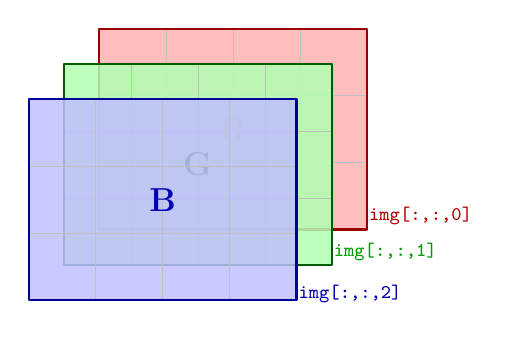
\begin{tikzpicture}[x={(-0.28cm,-0.28cm)}, y={(0.85cm,0cm)}, z={(0cm,0.85cm)},
                      line join=round]
    \def\W{4}
    \def\H{3}

    % Helper macro: draw one filled slice at depth \xx with given fill colour
    % Slices at x = 0 (R), 1 (G), 2 (B) — separated for clarity
    \foreach \xx/\fc/\lbl/\clr in {
        0/red!30/R/red,
        1.6/green!30/G/green!60!black,
        3.2/blue!25/B/blue}{
      % Fill
      \fill[\fc, opacity=0.85]
        (\xx,0,0) -- (\xx,\W,0) -- (\xx,\W,\H) -- (\xx,0,\H) -- cycle;
      % Grid
      \foreach \zz in {0,...,\H}
        \draw[gray!50, very thin] (\xx,0,\zz) -- (\xx,\W,\zz);
      \foreach \yy in {0,...,\W}
        \draw[gray!50, very thin] (\xx,\yy,0) -- (\xx,\yy,\H);
      % Border
      \draw[thick, \clr!60!black]
        (\xx,0,0) -- (\xx,\W,0) -- (\xx,\W,\H) -- (\xx,0,\H) -- cycle;
      % Channel label (centred on the face)
      \node[font=\large\bfseries, \clr!70!black] at (\xx, \W/2, \H/2) {\lbl};
    }

    % Annotation arrows pointing to each slice
    \node[font=\scriptsize, red!70!black]         at ( 0.0, \W+0.8, \H-2.8) {\texttt{img[:,:,0]}};
    \node[font=\scriptsize, green!60!black]       at ( 1.6, \W+0.8, \H-2.8) {\texttt{img[:,:,1]}};
    \node[font=\scriptsize, blue!70!black]        at ( 3.2, \W+0.8, \H-2.9) {\texttt{img[:,:,2]}};
  \end{tikzpicture}
\vspace{2mm}
\begin{card}{}
\centering
$x_c[m,n],\quad c\in\{R,G,B\}$\\[0.8mm]
$0\le m<H,\;\; 0\le n<W$\\[0.8mm]
$x_c[m,n]\in[0,255]$
\end{card}

\column{0.56\textwidth}
\centering
\img{0.8\linewidth}{figs/img/swirl.jpg}\\[1.5mm]
\img{0.26\linewidth}{figs/img/swirl_R.jpg}\hspace{1.5mm}%
\img{0.26\linewidth}{figs/img/swirl_G.jpg}\hspace{1.5mm}%
\img{0.26\linewidth}{figs/img/swirl_B.jpg}\\[1.2mm]
\begin{minipage}{0.84\linewidth}\centering
\capt{Indexing the third axis, \texttt{img[:,:,c]}, splits the photo into its R, G and B planes.}
\end{minipage}
\end{columns}
\end{frame}

% ------------------------------------------------------------------ 5  (S, 0:20)
\begin{frame}{Histograms: the statistics of each channel}
\vspace{2mm}
\begin{columns}[T,onlytextwidth]
\column{0.42\textwidth}
\begin{card}{Histogram of channel $\textit{\textcolor{accenttext}{c}}$}
\eqn{h_c[k] = \#\{(m,n) : x_c[m,n] = k\}}
\eqn{p_c[k] = \frac{h_c[k]}{H\,W},\qquad \sum_{k=0}^{255} p_c[k] = 1}
\end{card}
\vspace{1.5mm}
\begin{hotcard}{Perceived Luminance}
  \vspace{0.3em}
\eqn{Y = \begin{bmatrix} 0.299 & 0.587 & 0.114 \end{bmatrix}\begin{bmatrix} R \\ G \\ B \end{bmatrix}}
\vspace{0.3em}
{\scriptsize $Y$ uses the perceived luminance, which is closer to what the eye sees.}
\end{hotcard}
\column{0.55\textwidth}
\centering
\plot{0.86\linewidth}{hist.pdf}\\[1.5mm]
\begin{minipage}[c]{0.3\linewidth}\centering
\img{\linewidth}{figs/img/lakeside_sample.jpg}
\end{minipage}\hfill
\begin{minipage}[c]{0.66\linewidth}\raggedright
\capt{Lakeside sample (left). Blue sits highest (sky and water) and red lowest. The dashed curve is $Y$: narrower, because the channels are averaged inside every pixel.}
\end{minipage}
\end{columns}
\end{frame}

% ------------------------------------------------------------------ 6  (P, 0:25)
\begin{frame}{The 2D DFT: which frequencies build the picture}
\begin{columns}[T,onlytextwidth]
\column{0.43\textwidth}
\begin{card}{2D discrete Fourier transform}
\eqn{X[k,l] = \sum_{m=0}^{H-1}\sum_{n=0}^{W-1} x[m,n]\, e^{-j2\pi\left(\frac{km}{H}+\frac{ln}{W}\right)}}
\vspace{0.4em}
{\tiny \texttt{fftshift} puts DC in the centre; we display $\log(1+|X|)$}.
\end{card}\vspace{1mm}
\begin{card}{Parseval's theorem}
\eqn{\sum_{m,n}|x[m,n]|^2 = \frac{1}{HW}\sum_{k,l}|X[k,l]|^2}
\vspace{0.4em}
{\tiny Energy in space = Energy in frequency.}
\end{card}\vspace{1mm}
\begin{hotcard}{Partial reconstruction}
\eqn{\hat x = \big[\,\mathcal F^{-1}X_R,\;\; \mathcal F^{-1}X_G,\;\; 0\,\big]}
\end{hotcard}
\column{0.54\textwidth}
\centering
\lbl{LOG-MAGNITUDE SPECTRA, MEAN REMOVED}\\[0.8mm]
\img{0.25\linewidth}{figs/\figtheme/spec_R.png}\hspace{1.5mm}%
\img{0.25\linewidth}{figs/\figtheme/spec_G.png}\hspace{1.5mm}%
\img{0.25\linewidth}{figs/\figtheme/spec_B.png}\\[0.3mm]
\makebox[0.25\linewidth]{\lbl{R}}\hspace{1.5mm}\makebox[0.25\linewidth]{\lbl{G}}\hspace{1.5mm}\makebox[0.25\linewidth]{\lbl{B}}\\[1mm]
\lbl{INVERSE FFT OF CHOSEN CHANNELS}\\[0.8mm]
\img{0.25\linewidth}{figs/img/lake_clean.jpg}\hspace{1.5mm}%
\img{0.25\linewidth}{figs/img/recon_RG.jpg}\hspace{1.5mm}%
\img{0.25\linewidth}{figs/img/recon_GB.jpg}\\[0.3mm]
\makebox[0.25\linewidth]{\lbl{all three}}\hspace{1.5mm}\makebox[0.25\linewidth]{\lbl{R+G}}\hspace{1.5mm}\makebox[0.25\linewidth]{\lbl{G+B}}\\[0.5mm]
\begin{minipage}{0.85\linewidth}\centering\capt{Energy crowds at the centre (low frequencies).}\end{minipage}
\end{columns}
\end{frame}

% ------------------------------------------------------------------ 7  (P, 0:20)
\begin{frame}{Colour space: RGB $\rightarrow$ YCbCr is a change of basis}
\begin{columns}[T,onlytextwidth]
\column{0.52\textwidth}
\begin{card}{Full-range BT.601 transform}
\eqn{\begin{bmatrix} Y\\ C_b\\ C_r \end{bmatrix} =
\begin{bmatrix}
 0.299 & 0.587 & 0.114\\
-0.169 & -0.331 & 0.500\\
 0.500 & -0.419 & -0.081
\end{bmatrix}\!
\begin{bmatrix} R\\ G\\ B \end{bmatrix} +
\begin{bmatrix} 0\\ 128\\ 128 \end{bmatrix}}
\vspace{1em}
The $C_b$ and $C_r$ rows sum to zero, so a grey pixel ($R=G=B$) gets neutral chroma $128$.
\end{card}\vspace{1mm}
\begin{hotcard}{Why it helps}
R, G and B move together ($\rho_{RG}=0.994$ on this image). After the transform almost all the detail is in $Y$; $C_b$ and $C_r$ are smooth, so there is less to store.
\end{hotcard}
\column{0.45\textwidth}
\centering
\img{0.3\linewidth}{figs/img/ycc_Y.jpg}\hspace{1.2mm}%
\img{0.3\linewidth}{figs/img/ycc_Cb.jpg}\hspace{1.2mm}%
\img{0.3\linewidth}{figs/img/ycc_Cr.jpg}\\[0.3mm]
\makebox[0.3\linewidth]{\lbl{Y}}\hspace{1.2mm}\makebox[0.3\linewidth]{\lbl{Cb (contrast ×5)}}\hspace{1.2mm}\makebox[0.3\linewidth]{\lbl{Cr (contrast ×5)}}\\[1mm]
\plot{\linewidth}{energy_share.pdf}\\
\capt{Energy about the mean: \\ split evenly across R, G, B, but $98.9\%$ goes to $Y$.}
\end{columns}
\end{frame}

% ------------------------------------------------------------------ 8  (P, 0:25)
\section{Processing}
\begin{frame}{Filtering: convolution $\Leftrightarrow$ multiplication}
\begin{columns}[T,onlytextwidth]
\column{0.46\textwidth}
\begin{card}{2D convolution = LTI system}
\eqn{y[m,n] = \sum_{i}\sum_{j} h[i,j]\,x[m-i,\,n-j]}
\eqn{\Longleftrightarrow\quad Y[k,l] = H[k,l]\cdot X[k,l]}
\end{card}\vspace{1mm}
\begin{card}{Kernels are just different $h$}
  \vspace{0.3em}
\centering
\begin{tabular}{@{}c@{\hspace{5mm}}c@{}}
$\dfrac19\!\begin{bmatrix}1&1&1\\1&1&1\\1&1&1\end{bmatrix}$ &
$\begin{bmatrix}0&-1&0\\-1&5&-1\\0&-1&0\end{bmatrix}$\\[3.5mm]
\capt{box blur: low-pass, $\sum h=1$} & \capt{sharpen: $x-\nabla^2 x$}
\end{tabular}
\end{card}\vspace{1mm}
\begin{hotcard}{Gaussian and unsharp mask}
$G_\sigma\propto e^{-\frac{(i^2+j^2)}{2\sigma^2}}$, \; $y = x + a\,(x - G_\sigma * x)$\\[0.4mm]
$\Rightarrow$ one kernel: $h=(1+a)\,\delta - a\,G_\sigma$
\end{hotcard}
\column{0.51\textwidth}
\centering
\plot{0.95\linewidth}{freq_resp.pdf}\\[0.5mm]
\img{0.29\linewidth}{figs/img/filt_orig.jpg}\hspace{1.2mm}%
\img{0.29\linewidth}{figs/img/filt_gauss.jpg}\hspace{1.2mm}%
\img{0.29\linewidth}{figs/img/filt_unsharp.jpg}\\[0.3mm]
\makebox[0.29\linewidth]{\lbl{original}}\hspace{1.2mm}\makebox[0.29\linewidth]{\lbl{Gaussian, $\sigma{=}3$}}\hspace{1.2mm}\makebox[0.29\linewidth]{\lbl{unsharp, $a{=}1.5$}}\\[0.5mm]
\capt{Linear, so per-channel = whole-image ($\max|\Delta|<10^{-8}$).}
\end{columns}
\end{frame}

% ------------------------------------------------------------------ 9  (P, 0:25)
\begin{frame}{Denoising: the right filter depends on the noise}
\begin{columns}[T,onlytextwidth]
\column{0.43\textwidth}
\begin{card}{Two noise models}
Gaussian: \; $y = x + n,\;\; n\sim\mathcal N(0,\sigma^2)$\\[0.8mm]
S\&P: \; $y\in\{0,255\}$ with prob.\ $p$, else $x$
\end{card}\vspace{1mm}
\begin{card}{Median filter (non-linear)}
\eqn{y[m,n] = \operatorname{median}_{\,|i|,|j|\le 2}\; x[m+i,\,n+j]}
\vspace{0.5em}
\capt{A lone 0 or 255 is never the middle value, so it is dropped.}
\end{card}\vspace{1mm}
\begin{hotcard}[fontupper=\scriptsize\color{ink}]{Non-local means}
\eqn{\hat x(p) = \frac{\sum_q w(p,q)\,x(q)}{\sum_q w(p,q)}}
\eqn{w(p,q) = e^{-\frac{\|P_p-P_q\|^2}{h^2}}}
\end{hotcard}
\column{0.54\textwidth}
\centering
\lbl{GAUSSIAN NOISE, $\sigma=25$}\\[0.8mm]
\dn{dn_g_noisy}{}\hspace{0.8mm}\dn{dn_g_med}{}\hspace{0.8mm}\dn{dn_g_gb}{}\hspace{0.8mm}\dnb{dn_g_nlm}\\[0.3mm]
\makebox[0.225\linewidth]{\lbl{noisy 20.2 dB}}\hspace{0.8mm}\makebox[0.225\linewidth]{\lbl{median 30.0}}\hspace{0.8mm}\makebox[0.225\linewidth]{\lbl{Gaussian 30.3}}\hspace{0.8mm}\makebox[0.225\linewidth]{{\fontsize{6.5}{7.5}\selectfont\semifont\color{accenttext}NL-means 31.2}}\\[0.8mm]
\lbl{SALT \& PEPPER, $p=10\%$}\\[0.8mm]
\dn{dn_sp_noisy}{}\hspace{0.8mm}\dnb{dn_sp_med}\hspace{0.8mm}\dn{dn_sp_gb}{}\hspace{0.8mm}\dn{dn_sp_nlm}{}\\[0.3mm]
\makebox[0.225\linewidth]{\lbl{noisy 15.8 dB}}\hspace{0.8mm}\makebox[0.225\linewidth]{{\fontsize{6.5}{7.5}\selectfont\semifont\color{accenttext}median 35.8}}\hspace{0.8mm}\makebox[0.225\linewidth]{\lbl{Gaussian 26.2}}\hspace{0.8mm}\makebox[0.225\linewidth]{\lbl{NL-means 16.2}}\\[1mm]
\begin{minipage}{0.95\linewidth}\centering
  \vspace{1em}
\capt{PSNR vs.\ the clean crop ($5\times5$ windows, $h=15$).}
\end{minipage}
\end{columns}
\end{frame}

% ------------------------------------------------------------------ 10 (P, 0:25)
\section{Compression}
\begin{frame}{Lossy: keep only the strongest frequencies}
\begin{columns}[T,onlytextwidth]
\column{0.42\textwidth}
\begin{card}{Real image $\Rightarrow$ conjugate symmetry}
$X[k,l] = X^{*}[-k,\,-l]$ $\Rightarrow$ store only half.
\end{card}\vspace{1mm}
\begin{card}{Energy pruning, target $\eta$}
{\scriptsize Rank pairs by $E_p = w_p|X_p|^2$; keep the fewest (DC always) with}
\eqn{\sum_{p\in S} E_p \;\ge\; \eta \sum_{p} E_p}
\eqn{\hat x = \mathcal F^{-1}\{X\cdot\mathbf 1_S\}}
\end{card}\vspace{1mm}
\begin{hotcard}{Measuring the loss}
{\centering\resizebox{0.97\linewidth}{!}{$\displaystyle \mathrm{MSE}=\frac{1}{3HW}\sum (x-\hat x)^2,\quad \mathrm{PSNR}=10\log_{10}\frac{255^2}{\mathrm{MSE}}$}\par}
\end{hotcard}
\column{0.55\textwidth}
\centering
\plot{0.49\linewidth}{energy_curve.pdf}\hfill\plot{0.49\linewidth}{psnr_curve.pdf}\\[1mm]
\img{0.27\linewidth}{figs/img/lossy_90.jpg}\hspace{1.2mm}%
\img{0.27\linewidth}{figs/img/lossy_99.jpg}\hspace{1.2mm}%
\img{0.27\linewidth}{figs/img/lossy_99_9.jpg}\\[0.3mm]
\makebox[0.27\linewidth]{\lbl{$\eta{=}90\%$ \,$\cdot$\, 17.0 dB}}\hspace{1.2mm}\makebox[0.27\linewidth]{\lbl{$99\%$ \,$\cdot$\, 26.6 dB}}\hspace{1.2mm}\makebox[0.27\linewidth]{\lbl{$99.9\%$ \,$\cdot$\, 36.5 dB}}\\[0.5mm]
\capt{Our codec, $512\times512$ photo: $99\%$ of the energy is in $0.32\%$ of the coefficients. DC counts as energy, so detail returns near $99.9\%$.}
\end{columns}
\end{frame}

% ------------------------------------------------------------------ 10  (S, 0:25)
\begin{frame}{Lossless compression I: integer Haar lifting}
\begin{columns}[T,onlytextwidth]
\column{0.53\textwidth}
\begin{card}{Reversible colour transform (integers only)}
\eqn{\begin{bmatrix} R-G \\ G \\ B-G \end{bmatrix} =
\begin{bmatrix} 1&-1&0\\ 0&1&0\\ 0&-1&1 \end{bmatrix}
\begin{bmatrix} R \\ G \\ B \end{bmatrix},\qquad \det = 1}
\end{card}\vspace{1mm}
\begin{card}{Lifting one pair $(a,b)$}
\begin{tabular}{@{}p{0.45\linewidth}p{0.45\linewidth}@{}}
\semifont forward & \semifont exact inverse\\
$d = b-a$ & $a = s - \lfloor d/2 \rfloor$\\
$s = a + \lfloor d/2 \rfloor$ & $b = a + d$
\end{tabular}
\end{card}\vspace{1mm}
\begin{hotcard}{Example}
\centering
\begin{tikzpicture}[font=\small]
  \node (x) {$(10,\,14)$};
  \node[right=8mm of x] (y) {$(s,d)=(12,\,4)$};
  \node[right=8mm of y] (z) {$(10,\,14)$};
  \draw[flow] (x) -- node[above, font=\tiny, text=muted]{lift} (y);
  \draw[flow] (y) -- node[above, font=\tiny, text=muted]{undo} (z);
\end{tikzpicture}\\[0.3mm]
\capt{Smooth areas give $d\approx0$, and nothing is rounded away.}
\end{hotcard}
\column{0.44\textwidth}
\centering
\begin{tikzpicture}
  \node[inner sep=0] (h) {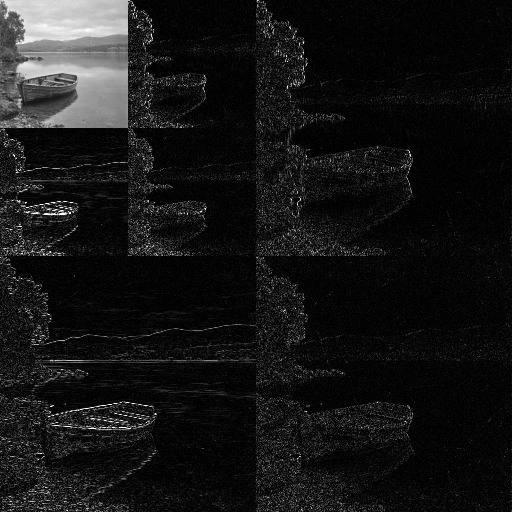
\includegraphics[width=0.72\linewidth]{figs/img/haar_subbands.jpg}};
  \draw[panelborder, line width=0.6pt] (h.south west) rectangle (h.north east);
  \coordinate (nw) at (h.north west); \coordinate (se) at (h.south east);
  \coordinate (c) at ($(nw)!0.5!(se)$);
  \coordinate (q) at ($(nw)!0.25!(se)$);
  \draw[accent, line width=0.7pt] (c |- nw) -- (c |- se) (c -| nw) -- (c -| se);
  \draw[accent, line width=0.5pt] (q |- nw) -- (q |- c) (q -| nw) -- (q -| c);
  \tikzset{bl/.style={font=\fontsize{6}{6}\selectfont\semifont, text=accenttext, fill=bg, fill opacity=0.8, text opacity=1, inner sep=0.5mm}}
  \node[bl, anchor=south east] at ($(se)+(-0.5mm,0.5mm)$) {HH$_1$};
  \node[bl, anchor=south east] at ($(c |- se)+(-0.5mm,0.5mm)$) {LH$_1$};
  \node[bl, anchor=south east] at ($(c -| se)+(-0.5mm,0.5mm)$) {HL$_1$};
  \node[bl, anchor=south east] at ($(c)+(-0.5mm,0.5mm)$) {HH$_2$};
  \node[bl, anchor=north west] at ($(nw)+(0.5mm,-0.5mm)$) {LL$_2$};
\end{tikzpicture}\\[1mm]
\begin{minipage}{0.8\linewidth}\centering
\capt{Two levels on our sample. Most detail is near zero (dark).}
\end{minipage}
\end{columns}
\end{frame}

% ------------------------------------------------------------------ 11  (S, 0:25)
\begin{frame}{Lossless compression II: coefficients to a \texttt{.iwv} file}
\vspace{5.5mm}
\centering
\begin{tikzpicture}[node distance=2.6mm, font=\fontsize{6.8}{8}\selectfont]
  \tikzset{st/.style={hot, inner sep=1.2mm, minimum height=9mm}}
  \node[box, inner sep=1.2mm, minimum height=9mm] (a) {RGB\\\capt{uint8}};
  \node[st, right=of a] (b) {Colour\\difference};
  \node[st, right=of b] (c) {Haar\\\capt{$L$ levels}};
  \node[st, right=of c] (d) {Zigzag\\\capt{to unsigned}};
  \node[st, right=of d] (e) {Byte\\planes};
  \node[st, right=of e] (f) {LZ77\\\capt{32 KiB window}};
  \node[st, right=of f] (g) {Huffman\\\capt{fixed codes}};
  \node[box, inner sep=1.2mm, minimum height=9mm, right=of g] (h) {\texttt{.iwv}\\\capt{+ CRC-32}};
  \foreach \u/\v in {a/b,b/c,c/d,d/e,e/f,f/g,g/h} \draw[flow] (\u) -- (\v);
  \draw[thin flow, rounded corners=1.5mm] (h.south) -- ++(0,-3.5mm) -| (a.south);
  \node[font=\fontsize{6.5}{7}\selectfont, text=muted, fill=bg, inner sep=0.8mm] at ($(a.south)!0.5!(h.south)+(0,-3.5mm)$) {decode runs every step in reverse, then the CRC must match: identical pixels};
\end{tikzpicture}
\vspace{0mm}
\begin{columns}[T,onlytextwidth]
\column{0.33\textwidth}
\begin{card}{Zigzag map}
\eqn{z = \begin{cases} 2c, & c \ge 0\\ -2c-1, & c<0 \end{cases}}
\capt{$0,-1,1,-2,2 \mapsto 0,1,2,3,4$: small magnitudes become small bytes.}
\end{card}\vspace{1mm}
\begin{card}{Entropy, bits per value}
\eqn{H = -\sum_v p(v)\log_2 p(v)}
\end{card}
\column{0.32\textwidth}
\centering
\plot{\linewidth}{coef_dist.pdf}\\
\capt{After the transform, $86\%$ of values lie within $\pm2$, so LZ77 and Huffman find far more repetition.}
\column{0.31\textwidth}
\begin{hotcard}{Result on a 256×256 crop}
\vspace{0.5em}
{\scriptsize
\renewcommand{\arraystretch}{1.1}
\begin{tabular}{@{}l@{\hspace{2mm}}r@{}}
Entropy (pixels) & 7.04 bits\\
Entropy (coefficients) & \hl{2.99 bits}\\
Raw RGB & 192.0 KiB\\
\texttt{.iwv} archive & \hl{112.0 KiB}\\
Ratio & \hl{1.71$\times$}\\
Decoded pixels & \hl{bit-exact}\\
\end{tabular}
}
\end{hotcard}
\end{columns}
\end{frame}

% ------------------------------------------------------------------ 12  (P, 0:25)
\section{Restoration}
\begin{frame}{Restoration: find the scratches, then fill them}
\begin{columns}[T,onlytextwidth]
\column{0.44\textwidth}
\begin{card}{Grey-scale morphology, $b$: $11\times11$ square}
\eqn{\begin{aligned}
f\ominus b &= \min_{b} f &&\text{erosion}\\
f\oplus b &= \max_{b} f &&\text{dilation}\\
f\circ b &= (f\ominus b)\oplus b &&\text{opening}\\
T(f) &= f - f\circ b &&\text{white top-hat}
\end{aligned}}
\end{card}\vspace{1mm}
\begin{hotcard}{Mask, then repair}
$M = \big[\,T(f)\ge\tau\,\big]\oplus (3\times3)$, \quad $\tau=30$\\[0.5mm]
Telea inpainting rebuilds the masked pixels from their neighbours. A mask over $10\%$ of the image is refused.
\end{hotcard}
\column{0.53\textwidth}
\centering
\begin{tikzpicture}[yscale=0.48, xscale=0.52]
  \draw[muted, line width=0.4pt] (0,0) -- (10.2,0);
  \fill[accent, opacity=0.3] (4.8,0) rectangle (5.2,1.6);
  \draw[third, line width=1.1pt] (0,1) -- (2,1.3) -- (4,1.5) -- (4.6,1.55) -- (4.8,3.2) -- (5.2,3.2) -- (5.4,1.6) -- (8,1.9) -- (10,1.7);
  \draw[accent, line width=1.1pt, dashed] (0,1) -- (2,1.3) -- (4,1.5) -- (5.4,1.6) -- (8,1.9) -- (10,1.7);
  \node[font=\fontsize{6.5}{7}\selectfont, text=third, anchor=west] at (5.7,3.1) {$f$: one row across a scratch};
  \node[font=\fontsize{6.5}{7}\selectfont, text=accenttext, anchor=west] at (5.7,2.45) {$f\circ b$: opening drops the thin peak};
  \node[font=\fontsize{6.5}{7}\selectfont, text=accenttext, anchor=west] at (5.7,0.6) {$T(f)$: only the scratch is left};
  \draw[accent, thin] (5.2,0.7) -- (5.7,0.6);
\end{tikzpicture}\\[1.5mm]
\img{0.235\linewidth}{figs/img/restore_before.jpg}\hspace{0.8mm}%
\img{0.235\linewidth}{figs/img/restore_tophat.jpg}\hspace{0.8mm}%
\img{0.235\linewidth}{figs/img/restore_mask.jpg}\hspace{0.8mm}%
\img{0.235\linewidth}{figs/img/restore_after.jpg}\\[0.3mm]
\makebox[0.235\linewidth]{\lbl{damaged}}\hspace{0.8mm}\makebox[0.235\linewidth]{\lbl{top-hat $T$}}\hspace{0.8mm}\makebox[0.235\linewidth]{\lbl{mask $M$}}\hspace{0.8mm}\makebox[0.235\linewidth]{\lbl{repaired}}\\[0.8mm]
\capt{The mask covers $1.6\%$ of the portrait. Bright hair highlights are picked up too, so a threshold slider controls the trade-off.}
\end{columns}
\end{frame}

% ------------------------------------------------------------------ 13  (P, 0:20)
\section{Results}
\begin{frame}{What Bindu delivers}
\vspace{2mm}
\begin{columns}[T,onlytextwidth]
\column{0.235\textwidth}
\begin{card}[height=21mm]{Decorrelation}
{\headfont\Large\color{accenttext}98.9\%}\\[0.5mm]of the variation moves into $Y$ after one $3\times3$ matrix.
\end{card}
\column{0.235\textwidth}
\begin{card}[height=21mm]{Fourier pruning}
{\headfont\Large\color{accenttext}0.32\%}\\[0.5mm]of the coefficients hold $99\%$ of the energy (26.6 dB).
\end{card}
\column{0.235\textwidth}
\begin{card}[height=21mm]{Wavelet codec}
{\headfont\Large\color{accenttext}1.71$\times$}\\[0.5mm]smaller than raw RGB, and decoded bit for bit.
\end{card}
\column{0.235\textwidth}
\begin{card}[height=21mm]{Restoration}
{\headfont\Large\color{accenttext}1.6\%}\\[0.5mm]of the pixels flagged and inpainted on the scratched portrait.
\end{card}
\end{columns}
\vspace{3mm}
\begin{columns}[c,onlytextwidth]
\column{0.5\textwidth}
\centering
\begin{tikzpicture}[font=\fontsize{6.5}{7.5}\selectfont]
  \node[hot, minimum width=17mm, minimum height=8mm, inner sep=1mm] (c) {\semifont Signals \&\\\semifont Systems};
  \foreach \a/\t in {90/Convolution, 25/Fourier analysis, -25/Decorrelation, -90/Wavelets, -155/Entropy, 155/Rate vs.\ distortion}{
    \node[box, minimum height=5.5mm, inner sep=1mm] (n\a) at (\a:26mm and 12mm) {\t};
    \draw[muted, line width=0.5pt] (c) -- (n\a);}
\end{tikzpicture}
\column{0.46\textwidth}
\begin{itemize}\setlength\itemsep{1.2mm}\footnotesize
  \item \hl{8 tools}: analysis, reconstruction, colour spaces, filters, noise lab, lossy and lossless codecs, scratch repair.
  \item Every result is \hl{measured}: PSNR, MSE, file sizes, entropy and exact-match checks.
  \item Limits: our pure-Python codec is slower than zlib, and repair masks are heuristic.
\end{itemize}
\end{columns}
\end{frame}

% ------------------------------------------------------------------ 14  (both, demo)
\section{Demo}
\begin{frame}[plain]
\centering
\vspace*{\fill}
{\color{accent}\rule{12mm}{1.5pt}}\\[4mm]
{\headfont\fontsize{30}{34}\selectfont\color{ink}Live demo}\\[3mm]
% {\semifont\color{accenttext}then your questions}\\[4mm]
{\color{accent}\rule{12mm}{1.5pt}}\\[8mm]
\begin{tikzpicture}[node distance=3mm]
  \node[box] (a) {1\;\; upload a photo};
  \node[box, right=of a] (b) {2\;\; spectra \& histograms};
  \node[box, right=of b] (c) {3\;\; compress / decompress};
  \node[box, right=of c] (d) {4\;\; repair scratches};
\end{tikzpicture}\\[10mm]
{\small\color{muted}Sajiid Jawad Talukder (2305041) \quad$\cdot$\quad Proteek Rosul (2305042)}
\vspace*{\fill}
\end{frame}
